%%%%%%%%%%%%%%%%%%%%%%%%%%%%%%%%%%%%%%%%%%%%%%%%%%%%%%%%%%%%%%%%%%%%%%%%%%%%%%%%%%%%%%%%%%%%%%%%%%%%%%%%%%%%%%
%%	Licencia:		Este documento se distribuye bajo licencia (CC BY 4.0) Usted puede encontrar un resumen %%
%%					de la licencia en http://creativecommons.org/licenses/by/4.0/deed.es					%%
%%																											%%
%%	-----------------------------------------------------------------------------------------------------	%%
%%																											%%
%%	Plantilla:		exi-examen																				%%
%%	Descripción:	exi-examen.tex es una plantilla para realizar exámenes escritos en formato LaTeX		%%
%%	Autor:			Ing. Alfonso Ramos Michel																%%
%%	Fecha:			9 de diciembre de 2013																	%%
%%	Revisión:		UNO-A																					%%
%%	Paquetes:		inputenc																				%%
%%					babel																					%%
%%					graphicx																				%%
%%					amsmath																					%%
%%					geometry 																				%%
%%					fancyhdr																				%%
%%	Comandos:		\ExiEscuela		Para definir la institución educativa donde se realiza el examen.		%%
%%					\ExiCarrera		Para definir la carrera que se realiza.									%%
%%					\ExiMateria		Para definir la materia que se cursa.									%%
%%					\ExiParcial		Para definir el parcial del cual se realiza el examen.					%%
%%					\informacion	Muesta un recuadro donde poder dar instrucciones al alumno.				%%
%%					\datos			Muestra una línea para el nombre del alumno y la fecha de realización.	%%
%%					\pregunta		Permite introducir (dentro del entorno enummerate) una pregunta o el 	%%
%%									planteamiento de un problema.											%%
%%%%%%%%%%%%%%%%%%%%%%%%%%%%%%%%%%%%%%%%%%%%%%%%%%%%%%%%%%%%%%%%%%%%%%%%%%%%%%%%%%%%%%%%%%%%%%%%%%%%%%%%%%%%%%




\documentclass[letterpaper,11pt]{article}

\usepackage[utf8]{inputenc}
\usepackage[spanish,mexico]{babel}
\usepackage{graphicx}
\usepackage{amsmath}
\usepackage{amsthm}
\usepackage{amsfonts}
%\usepackege{amssymb}
\usepackage[hmargin=1in, vmargin=1in]{geometry}
\usepackage{fancyhdr}
\pagestyle{fancy}
\usepackage{tasks}
\lhead{\ExiCarrera}
\chead{\ExiMateria}
\rhead{\ExiParcial}
\cfoot{\ExiEscuela}
\renewcommand{\headrulewidth}{0.4pt}
\renewcommand{\footrulewidth}{0.4pt}

\providecommand{\abs}[1]{\lvert#1\rvert}
\providecommand{\norm}[1]{\lVert#1\rVert}

%=================================================================================
%	Definición de comandos
%=================================================================================
\newcommand{\informacion}[1]{
\begin{center}
\fbox{\fbox{\parbox{\textwidth}{{\footnotesize#1}}}}
\end{center}
\vspace{5mm}}
\newcommand{\datos}{\makebox[0.7\textwidth]{Nombre:~\hrulefill} Fecha:~\hrulefill}
\newcommand{\pregunta}[2]{\item{#2}~{(#1 puntos)}\\ \vspace{5mm}						       
			{\bf Solución}}														  
%	Los siguientes comandos hay que definirlos desde aquí.								    %
\newcommand{\ExiCarrera}{Matemáticas para las Ciencias II.}											  %%%
\newcommand{\ExiMateria}{\textbf{Proyecto III}}														%%%%%%%%%%%%%%%%%%%%%%%%%%%%%
\newcommand{\ExiParcial}{Entrega: Viernes 20 de Marzo}														  %%%
\newcommand{\ExiEscuela}{\textbf{Facultad de Ciencias, UNAM}}	                		    %

%=================================================================================
%	Aquí comienza lo bueno, a definir el examen!!!!
%=================================================================================
\begin{document}



%%%%%%%%%%%%%%%%%%%%%            CARÁTULA            %%%%%%%%%%%%%%%%%%%%%%%%%
\setlength{\unitlength}{1cm}
\thispagestyle{empty}
\begin{picture}(18,4)
\put(-0.5,1.2){
\includegraphics[scale=.25]{unam1.png}}
\put(13.5,1){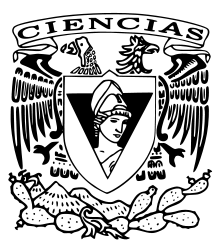
\includegraphics[scale=.35]{fciencias1.png}}
\end{picture}

\begin{center}
\vspace{-134pt}
\textbf{\large Matemáticas para las Ciencias II}\\[0.2cm]
\textbf{ Semestre 2020-2}\\[0.2cm]
Prof. Pedro Porras Flores\\[0.2cm]
Ayud. Irving Hérnandez Rosas \\ [0.2cm]
%Ayud. Carlos Rodolfo Barrera Anzaldot \\ [0.2cm]
\textbf{Proyecto III}
\end{center}
\vspace{-10pt}
\rule{17cm}{0.3mm}
\begin{flushright}
\vspace{-3pt}
\end{flushright}

%%%%%%%%%%%%%%%%%%%%%%%%%%%%%%%%%%%%%%%%%%%%%%%%%%%%%%%%%

%%%%%
%\informacion{\large Profesor: Pedro Porras  Flores \\
%porras@ciencias.unam.mx  \\

%Ayudante: María Guadalupe Gómez Farfán\\ 
 %lupis\_2309@hotmail.com\\
 
% Ayudante: Carlos Rodolfo Barrera Anzaldo\\ 
 %crba@ciencias.unam.mx\\}
%%%%
\noindent Realice los siguientes ejercicios, escribiendo el procedimiento claramente. Y recuerden que estos proyectos se entregan de manera individual en la plataforma de google classroom. 


\begin{enumerate}

% -----------------------------------------------------
% Problema uno
% -----------------------------------------------------

\item  Muestre que los siguientes conjuntos del plano son abiertos: 

\begin{tasks}(1)
\task $A = \{ (x,y) \in \mathbb{R} \vert - 1 < x < 1, - 1 < y < 1 \}$.
\task $B = \{ (x,y) \in \mathbb{R} \vert \,  0 < y  \}$.
\task $A = \{ (x,y) \in \mathbb{R} \vert \, 2 < x^2  + y^2 <  4 \}$.
\end{tasks}


\item  Calcule los siguientes. límites si existen: 

\begin{tasks}(3)
\task $\displaystyle\lim_{(x,y) \to (0,0)} \dfrac{\cos(xy) - 1}{x^2y^2}$.
\task $\displaystyle\lim_{(x,y) \to (0,0)} \dfrac{\sin(xy) }{xy}$.
\task $\displaystyle\lim_{x, \to 1} (x^2 , e^x) $.
\end{tasks}

\item  Usando la formulación $\epsilon$-$\delta$ muestre: 

\begin{tasks}(2)
\task $\displaystyle\lim_{(x,y,z) \to (0,0,0)} \dfrac{xyz}{x^2 + y^2 + z^2} = 0$.
\task $\displaystyle\lim_{(x,y) \to (0,0)} \dfrac{xy }{\sqrt{x^2 + y^2}} = 0$.
\task $\displaystyle\lim_{x, \to 2} (3x , x^2) = (6,4) $.
\end{tasks}
%\begin{figure}[h!]
%\centering
%\includegraphics[width=9cm]{silla}
%\caption{Parábola con foco sobre el eje $x$.}
%\label{F1}
%\end{figure}
\item  Sea $f: \mathbb{R}^2  \longrightarrow \mathbb{R}$ tal que $f(x,y) = \left\{
     \begin{array}{cl}
       \dfrac{x^2y}{\vert x \vert^3 + y^2} & : \text{ si } (x,y) \neq (0,0)\\
       0 & : \text{ si } (x,y) = (0,0)\\
     \end{array}
   \right.$. Muestre que $f$ continua es $(0,0)$.



\end{enumerate}




\end{document}
